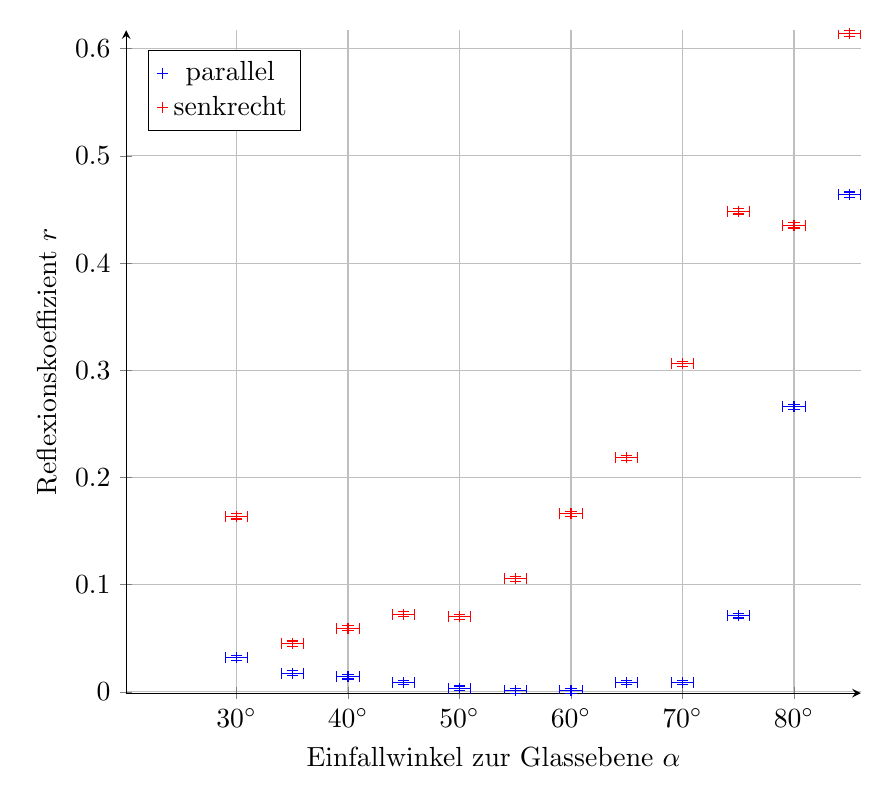
\begin{tikzpicture}
\begin{axis}[xticklabel=$\pgfmathprintnumber{\tick}^\circ$, width=.9\linewidth, height=10cm,
	axis y line=left, axis x line = bottom, xmin = 20.1, legend pos = north west,
	xmajorgrids = true,ymajorgrids = true,
	xlabel = {Einfallwinkel zur Glassebene $ \alpha $},
	ylabel = {Reflexionskoeffizient $ r $}]
	\addplot+ [only marks, mark=+, 
		error bars/.cd, x dir = both, x explicit,
		y dir = both, y explicit] 
	table[x=x,y=y, x error=xerr, y error=yerr] {
x	xerr	y	yerr
30	1	0.0317286652	0.002189285
35	1	0.0175054705	0.0021885191
40	1	0.0142231947	0.0021884051
45	1	0.0087527352	0.0021882676
50	1	0.0032822757	0.0021881956
55	1	0.0010940919	0.0021881851
60	1	0.0010940919	0.0021881851
65	1	0.0087527352	0.0021882676
70	1	0.0087527352	0.0021882676
75	1	0.0711159737	0.0021937102
80	1	0.2658643326	0.0022641981
85	1	0.4638949672	0.0024121673
	};
\addplot+ [only marks, mark=+, 
			error bars/.cd, x dir = both, x explicit,
			y dir = both, y explicit] 
		table[x=x,y=y, x error=xerr, y error=yerr] {
	x	xerr	y	yerr
	30	1	0.1637010676	0.002404058
	35	1	0.0450771056	0.0023748884
	40	1	0.059311981	0.0023766487
	45	1	0.0723606168	0.0023786824
	50	1	0.0699881376	0.0023782827
	55	1	0.1055753262	0.0023856646
	60	1	0.1660735469	0.0024049737
	65	1	0.2182680902	0.0024283353
	70	1	0.3060498221	0.0024811035
	75	1	0.4483985765	0.0026000698
	80	1	0.4353499407	0.0025875577
	85	1	0.6144721234	0.0027845832
		};
%	\addplot+[domain= -45:140, no marks, samples=100] {2043*(cos(x- 44.9940891727))^2};
\legend{parallel, senkrecht}
\end{axis}

\end{tikzpicture}